\documentclass[14pt, a4paper]{article}
\usepackage{fullpage}
\usepackage[top=2cm, bottom=2cm, left=2.5cm, right=2cm]{geometry}
\usepackage{amsmath,amsthm,amsfonts,amssymb,amscd}
\usepackage{fancyhdr}
\usepackage{fixltx2e}
\usepackage{mathrsfs}
\usepackage{listings}
\usepackage{color}
\usepackage{relsize}
\usepackage{graphicx}
\usepackage[utf8]{inputenc}
\usepackage[T1]{fontenc}
\usepackage[english, russian]{babel}

\definecolor{dkgreen}{rgb}{0,0.6,0}
\definecolor{gray}{rgb}{0.5,0.5,0.5}
\definecolor{mauve}{rgb}{0.58,0,0.82}

\DeclareMathSizes{14}{24}{18}{12}

\lstset{frame=tb,
  language=Python,
  aboveskip=3mm,
  belowskip=3mm,
  showstringspaces=false,
  columns=flexible,
  basicstyle={\small\ttfamily},
  numbers=none,
  numberstyle=\tiny\color{gray},
  keywordstyle=\color{blue},
  commentstyle=\color{dkgreen},
  stringstyle=\color{mauve},
  breaklines=true,
  breakatwhitespace=true,
  tabsize=3
}

\renewcommand{\thesection}{\arabic{section}.}
\renewcommand{\thesubsection}{\thesection\arabic{subsection}.}
\renewcommand{\thesubsubsection}{\thesubsection\arabic{subsubsection}.}

\begin{document}
\pagenumbering{gobble}
\begin{titlepage}
\begin{center}
\large{БЕЛОРУССКИЙ ГОСУДАРСТВЕННЫЙ УНИВЕРСИТЕТ 

ФАКУЛЬТЕТ ПРИКЛАДНОЙ МАТЕМАТИКИ И ИНФОРМАТИКИ

КАФЕДРА ВЫЧИСЛИТЕЛЬНОЙ МАТЕМАТИКИ}
\end{center}
\vspace*{\fill}
\begin{center}
Лабораторная работа 7

\large{\textbf{Метод наименьших квадратов приближения функции}}

Вариант 7
\end{center}
\begin{flushright}
\textbf{Выполнил:}

Журик Никита Сергеевич \\ 2 курс, 6 группа

\textbf{Преподаватель:}

Будник Анатолий Михайлович
\end{flushright}
\vspace*{\fill}
\begin{center}
Минск, 2019
\end{center}
\end{titlepage}

\tableofcontents
\newpage

\newpage
\pagenumbering{arabic}

  \section{Постановка задачи}
    \begin{enumerate}
      \item
      Посредством метода наименьших квадратов найти наилучшее среднеквадратичное приближение данной функции;
      \item
      Вычислить теоретическую оценку и действительную невязку интерполирования;
      \item
      Проанализировать полученные результаты.
    \end{enumerate}
  \section{Алгоритм решения}
  \begin{itemize}
     \item
     Рассмотрим приближение исходной таблично заданной функции $f(x) = 1.7e^{-x} - 0.7lnx, f(x) \in L_2[1, 2]$ алгебраическим многочленом степени не выше $n$: $P_n(x) = \sum\limits_{i = 0}^n c_ix^i$ на множестве точек $x_i = 1 + ih, i = \overline{1, N}, h = \frac{1}{N}, N = 10, n = 5$.
     \item
     Так как $L_2[1, 2]$ является гильбертовым пространством, элемент наилучшего приближения существует и единственный.
     \item
     Для нахождения коэффициентов $c_i$ составим СЛАУ путём скалярного умножения обеих частей равенства $f(x) = \sum\limits_{i = 0}^n c_ix^i$ на элементы базиса интерполирования $\phi_i(x) = x^i, i = \overline{1, n}$:
     \begin{equation}\begin{cases}(\phi_0, \phi_0)c_0 + (\phi_1, \phi_0)c_1 + \dots + (\phi_n, \phi_0)c_n = (f, \phi_0), \\ \vdots \\ (\phi_0, \phi_n)c_0 + (\phi_1, \phi_n)c_1 + \dots + (\phi_n, \phi_n)c_n = (f, \phi_n)\end{cases}\end{equation}
    Данная СЛАУ составлена относительна коэффициентов $c_i$ и имеет матрицу $A = [(x^i, x^j)]$, где $(x^i, x^j) = \sum\limits_{k = 0}^N x_k^ix_k^j$ в силу того, что исходная функция задана таблично. Вектор свободных членов состоит из скалярных произведений $(f, x^i) = \sum\limits_{k = 0}^N x_k^if(x_k)$.
    \item
    Решив указанную СЛАУ и подставив полученные коэффициенты в выражение для $P_n(x)$, получим искомое приближение функции алгебраическим многочленом степени не выше $n$.
    \item
    Для определения корректности поставленной задачи, а именно непрерывной зависимости решения от входных данных, найдём число обусловленности матрицы построенной СЛАУ, а именно матрицы Гильберта:
   \begin{equation}G_{n+1} = \begin{bmatrix}\frac{1}{1} & \frac{1}{2} & \dots & \frac{1}{n+1} \\ \frac{1}{2} & \frac{1}{3} & \dots & \frac{1}{n+2} \\ \vdots & \vdots & \ddots & \vdots \\ \frac{1}{n+1} & \frac{1}{n+2} & \dots & \frac{1}{2n+1}\end{bmatrix}\end{equation}
   В случае $n=5$: \begin{equation}\nu_{G_{n+1}} = 6.241533841033069 \cdot 10^{11}\end{equation}
   Следовательно, даже для $n = 5$ число обусловленности матрицы системы велико и задача поставлена не корректно, и погрешность во входных данных значительно изменит результат.
  \end{itemize}
  \section{Листинг программы}
  Для реализации алгоритма был использован Python и библиотеки numpy и matplotlib.

\begin{lstlisting}
#LeastSquares.py

import numpy as np
from math import exp, log, sqrt
import matplotlib.pyplot as plt

a = 1.0
b = 2.0
N = 10
n = 5
delta = (b - a) / N
alpha = 1.7

points = [a + i * delta for i in range(N + 1)]
c = np.zeros((n + 1, 1))

def l2scalar(f, g):
    values = [f(point) * g(point) for point in points]
    return np.sum(np.array(values, dtype=np.double))

def l2norm(f):
    return l2scalar(f, f)

def f(x):
    return alpha * exp(-x) + (1 - alpha) * log(x)

def phi(i):
    if i == n + 1:
        return f
    return lambda x: x ** i

def solution(x):
    global c
    value = 0.0
    for i in range(len(c)):
        value += c[i] * phi(i)(x)
    return value

def plotDifference(samples):
    space = np.linspace(a, b, samples)
    plt.plot(space, np.zeros(np.shape(space)))
    plt.plot(space, np.array([solution(x) - f(x) for x in space], dtype=np.double))
    plt.savefig("lsqDiff.png")
    plt.show()
    
if __name__ == '__main__':
    A = np.array([[l2scalar(phi(i), phi(j)) for j in range(len(c))] for i in range(len(c))],
                 dtype = np.double)
    B = np.array([l2scalar(f, phi(i)) for i in range(len(c))], dtype = np.double)
    c = np.linalg.solve(A, B)

    print("c:\n" + str(c))
    print()

    check = [points[0] + delta / 2.6, 
             points[5] + delta / 2.6,
             points[9] + delta / 2.6]
    
    detGN1 = np.linalg.det(A)
    print("Conditioning number: nu = " + str(np.linalg.norm(A, ord=np.inf) * np.linalg.norm(np.linalg.inv(A), ord=np.inf)))
    print()
    A = np.concatenate((A, np.array([B]).T), axis=1)
    A = np.vstack((A, np.array([l2scalar(f, phi(i)) for i in range(len(c) + 1)], dtype=np.double)))
    detGN2 = np.linalg.det(A)
    
    
    [print("rn({0}) = {1}".format(x, solution(x) - f(x))) for x in check]
    print()
    
    print("Expected deficiency: " + 
          str(sqrt(abs(detGN2 / detGN1))))
    
    space = np.linspace(a, b, 1000)
    print("Real deficiency on whole interval: " + 
          str(np.max(np.abs(np.array([(solution(x) - f(x)) for x in space], dtype=np.double)))))
    print()
    
    print("Real deficiency on control points: " + 
          str(np.max(np.abs(np.array([(solution(x) - f(x)) for x in check], dtype=np.double)))))
    
    plotDifference(1000)
\end{lstlisting}

  \section{Вывод программы}
\begin{verbatim}
c:
[ 3.04926117 -4.13112546  2.50490103 -1.01148796  0.23830349 -0.02445942]

Conditioning number: nu = 624153384103.3069

rn(1.0384615384615385) = 9.374749135870886e-06
rn(1.5384615384615385) = 4.441449420605759e-06
rn(1.9384615384615385) = 7.60907463800975e-06

Expected deficiency: 1.4694497815835233e-05
Real deficiency on whole interval: 1.0453241777508282e-05

Real deficiency on control points: 9.374749135870886e-06
\end{verbatim}
\begin{figure}[h!]
  \center
  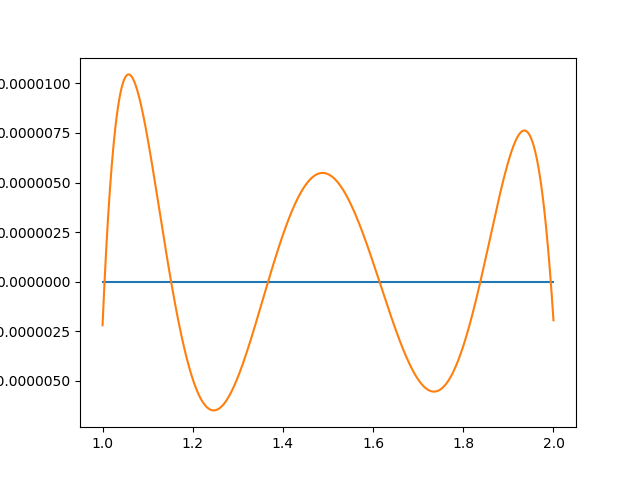
\includegraphics[width=0.6\linewidth]{lsqDiff.png}
  \caption{Невязка интерполирования}
\end{figure}

  \section{Выводы}
  \begin{itemize}
  \item
  Метод наименьших квадратов позволил приблизить исходную функцию с точностью $r_{LSQ_{real}} = \max\limits_x |r_n(x)| = 1.0453241777508282e-05$, что приблизительно совпадает с теоретической оценкой $r_{LSQ_{theor}} = 1.4694497815835233e-05$. Неточность вызвана тем, что исходная функция задана таблично, из-за чего скалярное произведение в пространстве $L2$ было заменено дискретным эквивалентом. В контрольных точках функция отклоняется не более, чем на $r_{LSQ_{control}} = 9.374749135870886e-06$.
  \item
  Глядя на график невязки, можно заметить, что невязка в середине отрезка меньше невязки на концах, что связано с тем, что за пределами отрезка интерполирования многочлен не совпадает с исходной функцией и невязка значительно увеличивается.
  \end{itemize}

\end{document}